\section{Supplemental}
\subsection{Reconstruction}

As the sample is rotated each detector pixel collects an intensity \(I(\theta) = I_{n}e^{-k(\theta)}\) at discrete (\(n\)) angles through a full rotation of the sample; where \(I_{n}\) is the unattenuated radiation intensity from the source to the detector, \(k\) is the attenuation caused by the sample along a detected ray an \(I(n)\) is the measured intensity, see \figurename~\ref{fig:OPT_digram}.
Rays from the sample to the detector approximate straight lines, and so the the rays reaching the detector with a line integrals.
A projection is then the resulting intensity profile at the detector for a rotation angle, and the integral transform that results in \(P_\theta(v)\)
% \(f(I_i,\theta_n) \)
is the \gls{Radon transform}.
% This is defined mathematically as:

\begin{align}
    \intertext{The equation of a set of parallel rays from a source passing through the specimen to a point \(v\) along the detector is:}
    &X\cos(\theta) + Y\sin(\theta) - v = 0 \\
    \intertext{Projecting many such rays through a sample with structure \(f(X,Y)\) gives:}
    P_\theta(v) = &\int_{\infty}^{\infty} \int_{\infty}^{\infty} f(X,Y)\delta (x\cos(\theta)+y \sin(\theta)-v)dX dY
\end{align}

% \begin{figure}
%     \centering
%     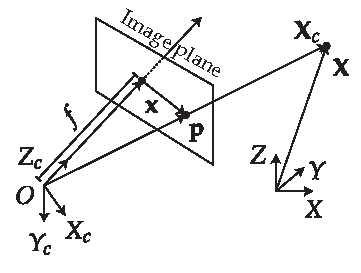
\includegraphics{coordinate_system}
%     \caption{Coordinate system}
%     \label{fig:coordinate_system_flopt}
% \end{figure}

Where \(P_\theta(v)\) is the \gls{Radon transform} of \(f(X,Y)\) which represents the contrast image of \gls{2D} slice of the specimen.
The \gls{Radon transform} of an image produces a \gls{sinugram} as in \figurename~\ref{fig:rawinputs}


% A parallel projection is then just the combination of line integrals  \(f(I) \) for a constant. % for a constant.

An inverse \gls{Radon transform} is used to recover the original object from the projection data; which is achieved by taking the \gls{Fourier transform} of each projection measurement, then reordering the information from the sample into the respective position in Fourier space.
This is valid due to the Fourier Slice theorem~\cite{bracewellStripIntegrationRadio1956} (see Appendix~\ref{appendix:fourierslice} for a derivation), which states that the \gls{Fourier transform} of a parallel projection is equivalent to a 2D slice of the Fourier transform of the original sample.
%A high pass filter such as a ramp filter is commonly used to counter the blurring caused by this oversampling.
% \gls{FBP} can be thought of as smearing the projection data across the image plane, and is expressed in equation form as:
\begin{align}
f_{\text{fpb}}(X,Y) = \int_{0}^{\pi} Q_\theta (X\cos(\theta)+Y\sin(\theta),\theta)dXdY
\end{align}

Where \(Q_\theta \) is the filtered projection data, and \(f_{\text{fpb}}(X,Y)\) is the back-projected image.
A spatial filtering step is applied during back-projection to avoid spatial frequency oversampling during the object’s rotation (see \figurename~\ref{fig:iradon_filter})
a high pass filter is commonly used to compensate for the perceived blurring.
The blurring arises as \(Q_\theta \) is back-projected (smeared) across the image plane for each angle of reconstruction; which means that not only does the back-projection contribute at the line it is intended to (along line \(C\) in \figurename~\ref{fig:coordinate_system_flopt}), but all other points along the back-projecting ray.
% The blurring occurs as \(Q_\theta\) makes the same contribution to the reconstruction for each angle
% will make the same contribution to the reconstruction at all of these points. Therefore, one could say that in the reconstruction process each filtered projection, Qe, is smeared back, or backprojected, over the image plane.


Now, suppose we know the relative positions of the two cameras and their respective intrinsic parameters, such as magnification and pixel offset.
For a single camera and given the camera parameters, we can translate pixel coordinates, \(\gls{w} = (u, v)\), into the coplanar image plane coordinates \(\gls{x}=(x, y)\):

\begin{align}
    u &= u_0 + k_u x \\
    v &= v_0 + k_v y
\end{align}

Knowing the focal length (\(f\)) of the imaging system, image plane coordinates may be projected into a ray in 3D.
The ray can be defined by using the point \gls{p} in camera-centred coordinates, where it crosses the image plane.

\begin{align}
  \mathbf{p} = \begin{bmatrix}
        x\\y\\z
      \end{bmatrix}
\end{align}

From the definition of a world point, as observed through an image, we can construct a dual-view model of world points in space as in \figurename~\ref{fig:epi-polar-geom}.
Using a model of a system with two views allows for the triangulation of rays based on image correspondences, this is an important part of stereo-vision.
The most important matching constraint which can be used the \emph{epipolar constraint}, and follows directly from the fact that the rays must intersect in 3D space.
Epipolar constraints facilitate the search for correspondences, they constrain the search to a 1D line in each image.
To derive general epipolar constraints, one should consider the epipolar geometry of two cameras as seen in \figurename~\ref{fig:epi-polar-geom}


The \textbf{baseline} is defined as the line joining the optical centres.
An \textbf{epipole} is the point of intersection of the baseline with the image plan and there are two epipoles per feature, one for each camera.
An \textbf{epipolar line} is a line of intersection of the epipolar plane with an image plane.
It is the image in one camera of the ray from the other camera’s optical centre to the world point (\gls{X}).
For different world points, the epipolar plane rotates about the baseline.
All epipolar lines intersect the epipole.

The epipolar line constrains the search for correspondence from a region to a line.
If a point feature is observed at \gls{x} in one image frame, then its location \gls{x'} in the other image frame must lie on the epipolar line.
We can derive an expression for the epipolar line.
The two camera-centered coordinate systems \gls{X_c'} and \gls{X_c} are related by a rotation, \gls{R} and translation, \gls{T} (see in \figurename~\ref{fig:epi-polar-geom}) as follows:

\begin{align}
    \gls{X_c'} &= \gls{R}\gls{X_c'} + \gls{T}
\end{align}
%       \\
%     \intertext{Taking the vector product with \(\gls{T}\), we obtain}
%     \gls{T} \times \gls{X_c'} &= \gls{T} \times \gls{R}\gls{X_c}+ \gls{T} \times \gls{T}  \\
%     \gls{T} \times \gls{X_c'} &= \gls{T} \times \gls{R}\gls{X_c}\label{eq:Xprime = RTX}
% \end{align}

\begin{figure}
  \centering
  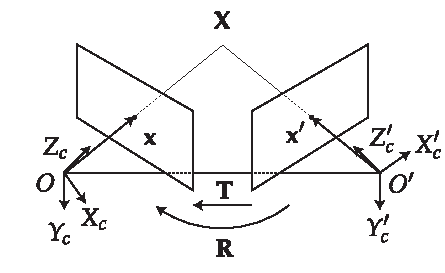
\includegraphics{./figures/epi-polar-geom}
  \caption[Epi-polar geometry described for two adjacent views]{
  Epi-polar geometry described for two adjacent views (or cameras of a scene).
  Coordinates as expressed in \figurename~\ref{fig:coordinate_system_flopt} with prime notation (\('\)) denoting the additional right camera view.
  Transforming from right to left camera-centered coordinates (\gls{X_c'} to \gls{X_c}) requires a rotation (\gls{R}) and a translation (\gls{T}).
  }\label{fig:epi-polar-geom}
\end{figure}

\subsection{The Essential matrix}

Taking the scalar product of \eqref{eq:Xprime = RTX} with \(\gls{X_c'}\), we obtain:
\begin{align}
    \gls{X_c'} \cdot (\gls{T} \times \gls{X_c}) &= \gls{X_c'}\cdot (\gls{T} \times \gls{R} \gls{X_c'}) \\
    \gls{X_c'} \cdot (\gls{T} \times \gls{R} \gls{X_c}) &= 0
    \intertext{A vector product can be expressed as a matrix multiplication:}
    \gls{T} \times \gls{X_c} &= \gls{T_x} \gls{X_c}
    \intertext{where}
    \gls{T_x} &=\begin{bmatrix}
    0    & -T_z  & T_y\\
    T_z  & 0     & -T_x\\
    -T_y  & T_x   & 0
    \end{bmatrix}
\end{align}
So equation~\eqref{eq:Xprime = RTX} can be rewritten as:

\begin{align}
\gls{X_c'} \cdot (\gls{T_x} \gls{R}\gls{X_c}) = 0 \\
\gls{X_c'} \gls{T} \gls{Essential} \gls{X_c}= 0 \\
\intertext{where}
\gls{Essential} = \gls{T_x} \gls{R}
\end{align}

\gls{Essential} is a \(3 \times 3\) matrix known as the \emph{essential matrix}.
The constraint also holds for rays \gls{p}, which are parallel to the camera-centered position vectors \gls{X_c}:

\begin{align}
\gls{p'}^T \gls{Essential} \gls{p} = 0 \label{eq:pEp}
\end{align}
This is the epipolar constraint.
If a point \gls{p} is observed in one image, then its position \gls{p'} in the other image must lie on the line defined by Equation~\eqref{eq:pEp}.
The essential matrix can convert from pixels on the detector to rays \gls{p} in the world, assuming a calibrated camera (intrinsic properties are known), and pixel coordinates can then be converted to image plane coordinates using:
\begin{align}
\begin{bmatrix}
u\\
v\\
1
\end{bmatrix}
&=
\begin{bmatrix}
k_u & 0 & u_0 \\
0 & k_v & v_0 \\
0 & 0 & 1
\end{bmatrix}
\begin{bmatrix}
x\\
y\\
1
\end{bmatrix}
\intertext{We can modify this to derive a relationship between pixel coordinates and rays:}
\begin{bmatrix}
u\\
v\\
1
\end{bmatrix}
&=
\begin{bmatrix}
\frac{k_u}{f} & 0 & \frac{u_0}{f} \\
0 & \frac{k_v}{f} & \frac{v_0}{f} \\
0 & 0 & \frac{1}{f}
\end{bmatrix}
\begin{bmatrix}
x\\
y\\
f
\end{bmatrix}
\intertext{\(\widetilde{\gls{K}}\) is defined as follows:}
\widetilde{\gls{K}} &= \begin{bmatrix}
f k_u & 0 & u_0 \\
0 & f k_v & v_0 \\
0 & 0 & 1
\end{bmatrix}
\intertext{then we can write pixel coordinates in homogenous coordinates:}
\widetilde{\gls{w}} &= \widetilde{\gls{K}} \gls{p}
\end{align}

\subsection{The Fundamental matrix}

\begin{align}
    \intertext{From~\eqref{eq:pEp} the epipolar constraint becomes}
    % \mathbf{p'}^T E \mathbf{p} &= 0 \\
    \widetilde{\gls{w'}} ^T \widetilde{\gls{K}}^{-T} E \widetilde{\gls{K}}^{-1} \widetilde{\gls{w}}  &= 0 \\
    \widetilde{\gls{w'}} ^T F \widetilde{\gls{w}}  &= 0
\end{align}
%\subsubsection{Two views}
%\paragraph{Mapping from one camera to another}
%\subsubsection{Three and more views}
The (\(3\times3)\) matrix \gls{F}, is the called the \emph{fundamental matrix}.
With intrinsically calibrated cameras, structure can be recovered by triangulation.
First, the two projection matrices are obtained via a \gls{SVD} of the essential matrix.
The \gls{SVD} of the essential matrix is given by:

\begin{align}
    \gls{Essential} &= \gls{K'}^T \gls{F} \gls{K} = \gls{T_x} \gls{R} = \mathbf{U}\Lambda \mathbf{V}^T\\%\gls{R} = U\LambdaV^T\\
    \intertext{It can be shown that}
    \hat{\gls{T_x}} &= U \begin{bmatrix}
    0 & 1 & 0 \\
    -1 & 0 & 0 \\
    0 & 0 & 0
    \end{bmatrix} U^T
    \intertext{ and }
    \gls{R} &= U \begin{bmatrix}
    0 & -1 & 0 \\
    1 & 0 & 0 \\
    0 & 0 & 1
    \end{bmatrix} V^T
    \intertext{Then, aligning the left camera and world coordinate systems gives the projection matrices:}
    \mathbf{P} &= \gls{K}    \begin{bmatrix}[c|c]       \mathbf{I} & \mathbf{0}   \end{bmatrix}
    \intertext{ and }
    \mathbf{P}' &= \gls{K'} \begin{bmatrix}[c|c]       \gls{R} & \gls{T}   \end{bmatrix}
\end{align}
Where \( \begin{bmatrix}[c|c] \mathbf{I} & \mathbf{0} \end{bmatrix}\) is the identity matrix augmented column-wise with a zero matrix, and the two projection matrices (\(\mathbf{P}\) and \(\mathbf{P}'\)) project from camera pixel coordinates to world coordinates.
Given these projection matrices, scene structure can be recovered (only up to scale, since only the magnitude of \gls{T} (|\gls{T}|) is unknown) using least squares fitting.
Ambiguities in \gls{T} and \gls{R} are resolved by ensuring that visible points lie in front of the two cameras.
As with the essential matrix, the fundamental matrix can be factorised into a skew-symmetric matrix corresponding
to translation and a \(3 \times 3\) non-singular matrix corresponding to rotation.



\begin{figure}
  \centering
   \hspace*{\fill}
  \begin{subfigure}[t]{0.3\textwidth}
    
\includegraphics[width=\textwidth]{./figures/results/no_helix/iradon_nofilter}
    \caption[Unfiltered iRadon]{This is the unfiltered reconstruction of the object using the \gls{Radon transform}}%TODO equation???
    \label{fig:iradon_nofilter}
  \end{subfigure}\hfill
  \begin{subfigure}[t]{0.3\textwidth}
    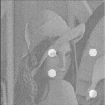
\includegraphics[width=\textwidth]{./figures/results/no_helix/iradon_filter}
    \caption[Filtered iRadon]{Ram-lak (Fourier ramp) filter applied to \figurename~\ref{fig:iradon_nofilter}.}
    \label{fig:iradon_filter}
  \end{subfigure}
     \hspace*{\fill}
    % \label{fig:irandons}
  \caption{The result of a tomographic reconstruction (using equally spaced angular steps and no translation between frames) requires Fourier filtering to normalise spatial contrast.}\label{fig:irandons}%TODO simulations with no drift and skew and use equation
\end{figure}

The second approach is less prone to compound errors but relies on precise identification and tracking of fiducial markers.
distinction and tracking fiducials.
Instead of calculating \gls{F} between neighbouring images, \gls{F} is calculated between the current projection and the very first projection.
\gls{F} is then decomposed and the transformation matrix is inverted and applied to the back projected volume.
The reoriented back projected volumes are summed and finally filtered to remove the additional spatial frequencies imparted from rotating the sample.

% \subsection{Bead tracking}

% \section{Future work}
%
% \subsection{Bead tracking}
% The work presented here is, so far, is a proof-of-concept demonstrated by simulation and reconstruction from ground-truth testcard objects, and requires several further steps in order apply it to real \gls{OPT} data.
% Firstly, a bead-tracking algorithm~\cite{crockerMethodsDigitalVideo1996} will need to be created to reliably track multiple beads, concurrently, in an image series.
% A sensible approach would be to have a user select the fiducial markers in the image on the first frame and template match in a small window around the selection; this is similar to the algorithm described in Chapter~\ref{chapter:spt}.
% Template matching is robust to occlusions provided the fiducial is not fully eclipsed.
% If two fiducial markers occlude each other however, this algorithm may switch their identities or both tracking windows may follow one bead.
% This is a common problem in particle tracking algorithms, but is solved by using a weighted likelihood based on momentum\cite{chenouardMultipleHypothesisTracking2013}.
%
% The likelihood of a bead occlusion occurring will increase with he introduction of additional beads into the sample.
% As such occluded beads may need to be omitted. % and possibly interpolated for.

% Egregious outliers may be found by tracking a \emph{confidence} estimator as the bead rotates as in
% A primitive estimator would be the pixel-wise sum of intensities in the result of a correlative template matching.
% Whilst this confidence value itself has no physical interpretation, any stark changes in the derivative will be suggestive of an occlusion or mis-tracking of some variety, see \figurename~\ref{fig:confidence_bead_tracking}.

% \begin{figure}
%   \centering
%   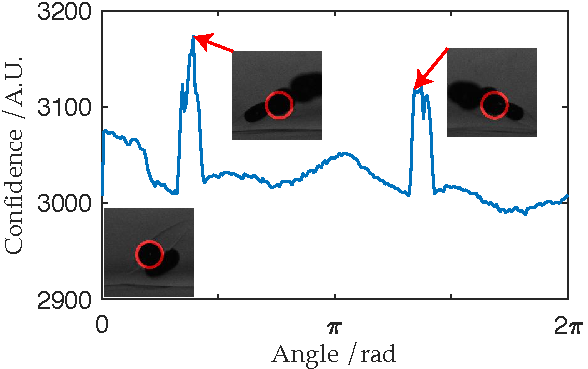
\includegraphics{./figures/results/confidence_bead_tracking}
%   \caption{A plot of the confidence value of a single fiducial bead being tracking \emph{in vivo}.
%   Sharp changes in the confidence value occur when the fiducial bead is occluded.
%   The image at the origin shows the fiducial being tracked well in the first frame.
%   (Images courtesy of Pedro Vallejo)
%   }
%   \label{fig:confidence_bead_tracking}
% \end{figure}

% \subsection{Multiple views tracking}
% The theory backing the proposed algorithm relies on triangulation between two view points.
% In this work the two view points refer to the image at frames \(n\) and \(n+1\).
% However, it is possible to use three separate views (frames \(n\), \(n+1\) and \(n+2\)) to reconstruct a scene, one such approach being quaternion tensors.
% Working with tensors is computationally and mathematically more challenging, but a future iteration of the algorithm presented here may benefit from using three views to provide a more accurate transformation matrix.
% Beyond three views there currently is no mathematical framework at present for four or more views.
% If such tools did exist, it may be possible to make the algorithm described above as non-iterative and essentially a single shot reconstruction from pixels to voxels.

% \subsection{Fiducial free reconstruction}
%
% In computer vision, scenes often do not contain known fiducial marks and so such marks are found between views.
% To find such a correspondences, points with similar local texture are found and matched in between each image. %, many of these such correspondences are found
% This technique is only valid for views with small angles between them, as would be found in \gls{OPT}.
% A similar method could be introduced into the algorithm presented here, as each image should have sufficient texture, particularly when using \gls{tOPT}.
%
% The following chapter will move from improvements in registration using projective matrices and into improvements in resolution using on-camera slit-scanning.

%A future version of this algorithm may be able to use 3 views to produce a more faithful transformation matrix.
%The mathematics for more than three views currently does not exist.


\begin{figure}
  \centering
  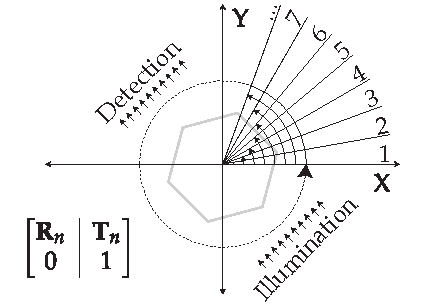
\includegraphics{./figures/flOPT_principle}
  \caption[Principles of the proposed algorithm]{Principles of the proposed algorithm. Each successive frame of \gls{OPT} image data will have an associated \gls{R} and \gls{T} (shown here in augmented form using homogenous coordinates), these matrices can be recovered from comparing the fiducial marker positions in each frame (\(n\)) and its successor (\(n+1\)).}
\end{figure}



\begin{figure}
  \centering
   \hspace*{\fill}
  \begin{subfigure}[t]{0.3\textwidth}
    \begin{tikzpicture}[node distance=0cm]
      \node (img) {
\includegraphics[width=0.8\textwidth]{./figures/results/no_helix/iradon_nofilter}};
       \node[below=of img] {\(X\)};
       \node[left=of img,rotate=90,yshift=0.2cm] {\(Y\)};
    \end{tikzpicture}
    \caption[Unfiltered iRadon]{This is the unfiltered reconstruction of the object using the \gls{Radon transform}}\label{fig:iradon_nofilter}%TODO equation???
  \end{subfigure}\hfill
  \begin{subfigure}[t]{0.3\textwidth}
    \begin{tikzpicture}[node distance=0cm]
      \node (img) {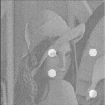
\includegraphics[width=0.8\textwidth]{./figures/results/no_helix/iradon_filter}};
       \node[below=of img] {\(v\)\vphantom{\(X\)}};
       \node[left=of img,rotate=90,yshift=0.2cm] {\(Y\)};
    \end{tikzpicture}
    \caption[Filtered iRadon]{Ram-lak (Fourier ramp) filter applied to \figurename~\ref{fig:iradon_nofilter}.}\label{fig:iradon_filter}
  \end{subfigure}
   \hspace*{\fill}
  \caption[Effects of filtering the result of a inverse Radon transform reconstruction]{
  The result of a tomographic reconstruction (using equally spaced angular steps and no translation between frames) requires Fourier filtering to normalise spatial contrast.}\label{fig:irandons}%TODO simulations with no drift and skew and use equation
\end{figure}


\begin{figure}
  \centering
   \hspace*{\fill}
  \begin{subfigure}[t]{0.3\textwidth}
    \begin{tikzpicture}[node distance=0cm]
      \node (img) {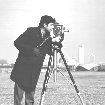
\includegraphics[width=0.8\textwidth]{./figures/results/no_helix/flopt_camerman}};
       \node[below=of img] {\(Z\)};
       \node[left=of img,rotate=90,yshift=0.2cm] {\(Y\)};
    \end{tikzpicture}
    \caption{Filtered reconstruction Cameraman testcard}
  \end{subfigure}\hfill
  \begin{subfigure}[t]{0.3\textwidth}
    \begin{tikzpicture}[node distance=0cm]
      \node (img) {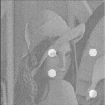
\includegraphics[width=0.8\textwidth]{./figures/results/no_helix/flopt_filter}};
       \node[below=of img] {\(X\)};
       \node[left=of img,rotate=90,yshift=0.2cm] {\(Y\)};
    \end{tikzpicture}
    \caption{Filtered reconstruction of Lena testcard}
  \end{subfigure}
   \hspace*{\fill}
   \caption[Filtered reconstruction of the ground truth reference image using the new proposed algorithm.]{
  Filtered reconstruction of the ground truth reference image from \figurename~\ref{fig:recon_iterative} using the new proposed algorithm.
  }\label{fig:flopt_filter}
\end{figure}



\begin{figure}
  \centering
   \hspace*{\fill}
  \begin{subfigure}[t]{0.3\textwidth}
    \begin{tikzpicture}[node distance=0cm]
      \node (img) {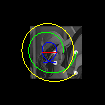
\includegraphics[width=0.8\textwidth]{./figures/results/helix/topdown_bead_paths}};
       \node[below=of img] {\(X\)};
       \node[left=of img,rotate=90,yshift=0.2cm] {\(Y\)};
    \end{tikzpicture}
    \caption{Top down views (\(X,Y\)) of the source image with the fiducial paths marked.}\label{fig:topdown_bead_paths}
  \end{subfigure}\hfill
  \begin{subfigure}[t]{0.3\textwidth}
    \begin{tikzpicture}[node distance=0cm]
      \node (img) {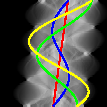
\includegraphics[width=0.8\textwidth]{./figures/results/helix/sinugram_stretch}};
       \node[below=of img] {\(v\)\vphantom{\(X\)}};
       \node[left=of img,rotate=90,yshift=0.2cm] {\(n\)};
    \end{tikzpicture}
    \caption{Sinugram (\(v,n\)) of a sample whose axis of rotation has a systematic drift}\label{fig:flopt_helix_sinugram}
  \end{subfigure}
   \hspace*{\fill}
   \caption{Comparison of the two reconstructions under sample imaging with a systematic drift, in 3D though represented here in 2D.}\label{fig:flopts}
\end{figure}

\begin{figure}
  \centering
   \hspace*{\fill}
  \begin{subfigure}[t]{0.3\textwidth}
    \begin{tikzpicture}[node distance=0cm]
      \node (img) {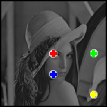
\includegraphics[width=0.75\textwidth]{./figures/results/no_helix/rawinput_colour}};
       \node[below=of img] {\(X\)};
       \node[left=of img,rotate=90,yshift=0.2cm] {\(Y\)};
    \end{tikzpicture}
    \caption{Ground truth image for \gls{OPT} simulations, Lena (\(f(X, Y)\)).}\label{fig:raw_input}
  \end{subfigure}\hfill
  \begin{subfigure}[t]{0.3\textwidth}
    \begin{tikzpicture}[node distance=0cm]
      \node (img) {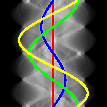
\includegraphics[width=0.8\textwidth]{./figures/results/no_helix/sinugram_stretch}};
       \node[below=of img] {\(v\)\vphantom{\(X\)}};
       \node[left=of img,rotate=90,yshift=0.2cm] {\(\theta\)};
    \end{tikzpicture}
    \caption{Image of Lena (\figurename~\ref{fig:raw_input}) after rotation and projection in 2D, giving the \gls{sinugram} (\(P_{\theta}(v)\)).
    }\label{fig:sinugram_stretch}
  \end{subfigure}
   \hspace*{\fill}
  \caption{Reference images for \gls{OPT} reconstruction.}\label{fig:rawinputs}
\end{figure}
